\section{Experimental Results}
\label{sec:moe_results}
We demonstrate the efficacy of the mixture of expert controllers in simulation
and real-world experiments.
%
In the first case study, we learn a gating network that switches between two
unstable closed-loop systems to result in a piecewise-stable system.
%
Then, we find switching expert controllers for the cartpole system enclosed with
wall barriers.
%

\subsection{Stable Switching Between Unstable Systems}

Suppose we have two linear closed-loop systems of the form 
\begin{equation}
    \begin{gathered}
        \dot{x} = A_1x = \bmat{0 & -1 \\ 2 & 0}x \\
        \dot{x} = A_2x = \bmat{0 & -2 \\ 1 & 0}x.
    \end{gathered}
    \label{eq:unstable_closedloop}
\end{equation}
%
Even if both systems are unstable, it is possible to find a state-dependent
switching rule that makes the resulting switched system
stable~\cite{liberzon2003switching}. 
%
We aim to learn the parameters $\psi$ of the gating network $P(x;
\psi)$ such that the switching system converges to the desired equilibrium $x^*
= (0, 0)$.
%
The gating network is a fully-connected neural net with one hidden layer ($2
\rightarrow 6 \rightarrow 4$ neurons) and an \textsc{Elu} activation
function~\cite{clevert2015fast}.
%
We constrain the maximum number of state partitions to $4$.
%
Each state partition has a corresponding controller parameter $\theta_i \in
\mathbb{R}$. 
%
The control law is a sample from the Bernoulli probability distribution
\begin{align}
    u(\theta_i) = \begin{cases}
       0, & \theta_i > \frac{1}{2}, \\
       1, & \theta_i \leq \frac{1}{2},
    \end{cases}
\end{align}
\noindent where $u = 0$ corresponds to the first dynamics $\dot{x} = A_1
x$ and $u=1$ corresponds to $\dot{x} = A_2x$.
%
We use the \textsc{Sigmoid} activation function to limit $\theta_i$ between 0
and 1.
%
We generate a trajectory following the procedure in
Algorithm~\eqref{algo:switching_A1A2}.
%
The likelihood is modified to account for the probabilistic control as
\begin{align*}
    \mathbb{L}(\phi) = \int_{0}^{T} \Biggl( \sum_{i=1}^{N_F} - \theta_i \ell \Bigl(x(t), u(\theta_i) \Bigr) - (1- \theta_i)\ell \Bigl(x(t), u(1-\theta_i) \Bigr) +
    \ln  P\Bigl(c_i = i | x(t), \psi \Bigr)  \Biggr) \dd t.
\end{align*}

\begin{algorithm}
    \setstretch{1.2}
      \caption{Stable Switching between Unstable Systems}
      \label{algo:switching_A1A2}
      \small
      \hspace*{\algorithmicindent} \textbf{Input}: $x(0) = (q(0), \dot{q}(0))$
      \begin{algorithmic}[1]
        \State $\phi \leftarrow  [z(0)]$ \Comment{Initial States}
          % \algrenewcommand\algorithmicindent{0em} % No indent
            \For{$t \in 0:\Delta t:T$} 
              \State $i \sim \text{Categorical}\Bigl(P(x(t); \psi)\Bigr)$ \Comment{Sample a bin number}
              \State $u \sim \text{Bernoulli} \Bigl(\textrm{Sigmoid}(\theta_i) \Bigr)$      
              \State $x(t+\Delta t) = (1-u)A_1x(t) + u \; A_2x(t) $
              \State $\phi \leftarrow \phi \cup [x(t+\Delta t)]$
            \EndFor
          \State \textbf{return} $\phi$
      \end{algorithmic}
  \end{algorithm}
  
The resulting switching system is shown in Figure~\ref{fig:switching_plot}.

%%%%%%%%%%%%%%%%%%%%%%%%%%%%%%%%%%%%%%%%%%%%%%%%%%%%%%%%%%%%%%%%%%%%%%%%%%%%%%%%%%%%%%%%
\subsection{Cartpole with Wall Contacts}
\label{ssec:cartpole_with_walls}

In this section, we take the classical cartpole swing-up problem and introduce
contact events from two barriers as shown Figure~\ref{fig:cartpole}. 
%
We demonstrate the performance of the mixture of expert controllers in
simulation and real-world experiments.
%
Lastly, we compare the performance of the mixture of expert controllers against
a single swing-up controller. 


\subsubsection{System Model}
\label{sssec:cartpole_model}

The cartpole system consists of a freely rotating pendulum link, riding on an
actuated cart.
%
The setup is enclosed by two rigid walls hanging $0.2$m from the bottom of the
cart.
%
The objective is to use the control authority on the cart in order to swing-up
the passive pendulum to the upright.
%
The pendulum spans length of $l=0.2$m and its mass $m_c = 0.75$kg is
concentrated at the distance $l_{cm}=\nicefrac{l}{2}$ from the hinge.
%
The cart alone has a mass of $m_p=0.165$ kg. The viscous friction between the
cart and the track its sliding on is characterized by the coefficient $b=1.2$
\nicefrac{N $\cdot$ sec}{m}.
%
The dynamics of the system
is given by~\eqref{eq:hybrid_dynamics} where 
\begin{equation}
    \begin{gathered}
        M(q) = \bmat{m_c + m_p & -m_p+l_{cm} \cos(\theta) \\
        -m_pl_{cm}\cos(\theta) & m_p l_{cm}^2+I_1} \\
        C(q, \dot{q}) = \bmat{b  & m_pl_{cm}\sin(\theta) \\
                -m_p\sin(\theta)/2 & 0} \\
        G(q) = \bmat{0 & -m_pg l_{cm} \sin(\theta)}^\top \\
        B = [1 \; 0]^\top
    \end{gathered}
\end{equation}
\noindent where $q = [x_c; \theta]$, $x_c$ is the location of the cart and
$\theta$ is the angle of the pendulum from the vertical. 
%
There are a total of $k=10$ contact events between the pendulum and the sides of
the walls.
%
We integrate closed-loop trajectories with Moreau time stepping algorithm
outlined in Algorithm~\eqref{algo:moreau} with an integration time step $\Delta
t=0.001$.
%

\subsubsection{Training}
\label{sssec:cartpole_training}

The goal is to learn mixture of expert controllers to stabilize the system at
$x^* = (q^*, \dot{q})^* = (0, 0)$.
%
Once the system reaches within a small neighborhood of $x^*$, we employ Linear
Quadratic Regulator (LQR) to stabilize at the desired equilibrium.
%
We use minimum trajectory loss (MTL) discussed in
Section~\ref{sssec:performance_objective} with time horizon $T=1.5$s.
%
In each parameter update, we sample $N_{\mathcal{D}}=4$ initial states through
greedy and explorative techniques.
%


\begin{figure}[H]
    \centering
    \includegraphics[width=0.7\linewidth]{MOEfirstImpact.png}
    \label{fig:cartpole}
\end{figure}

\begin{figure}[H]
    \centering
    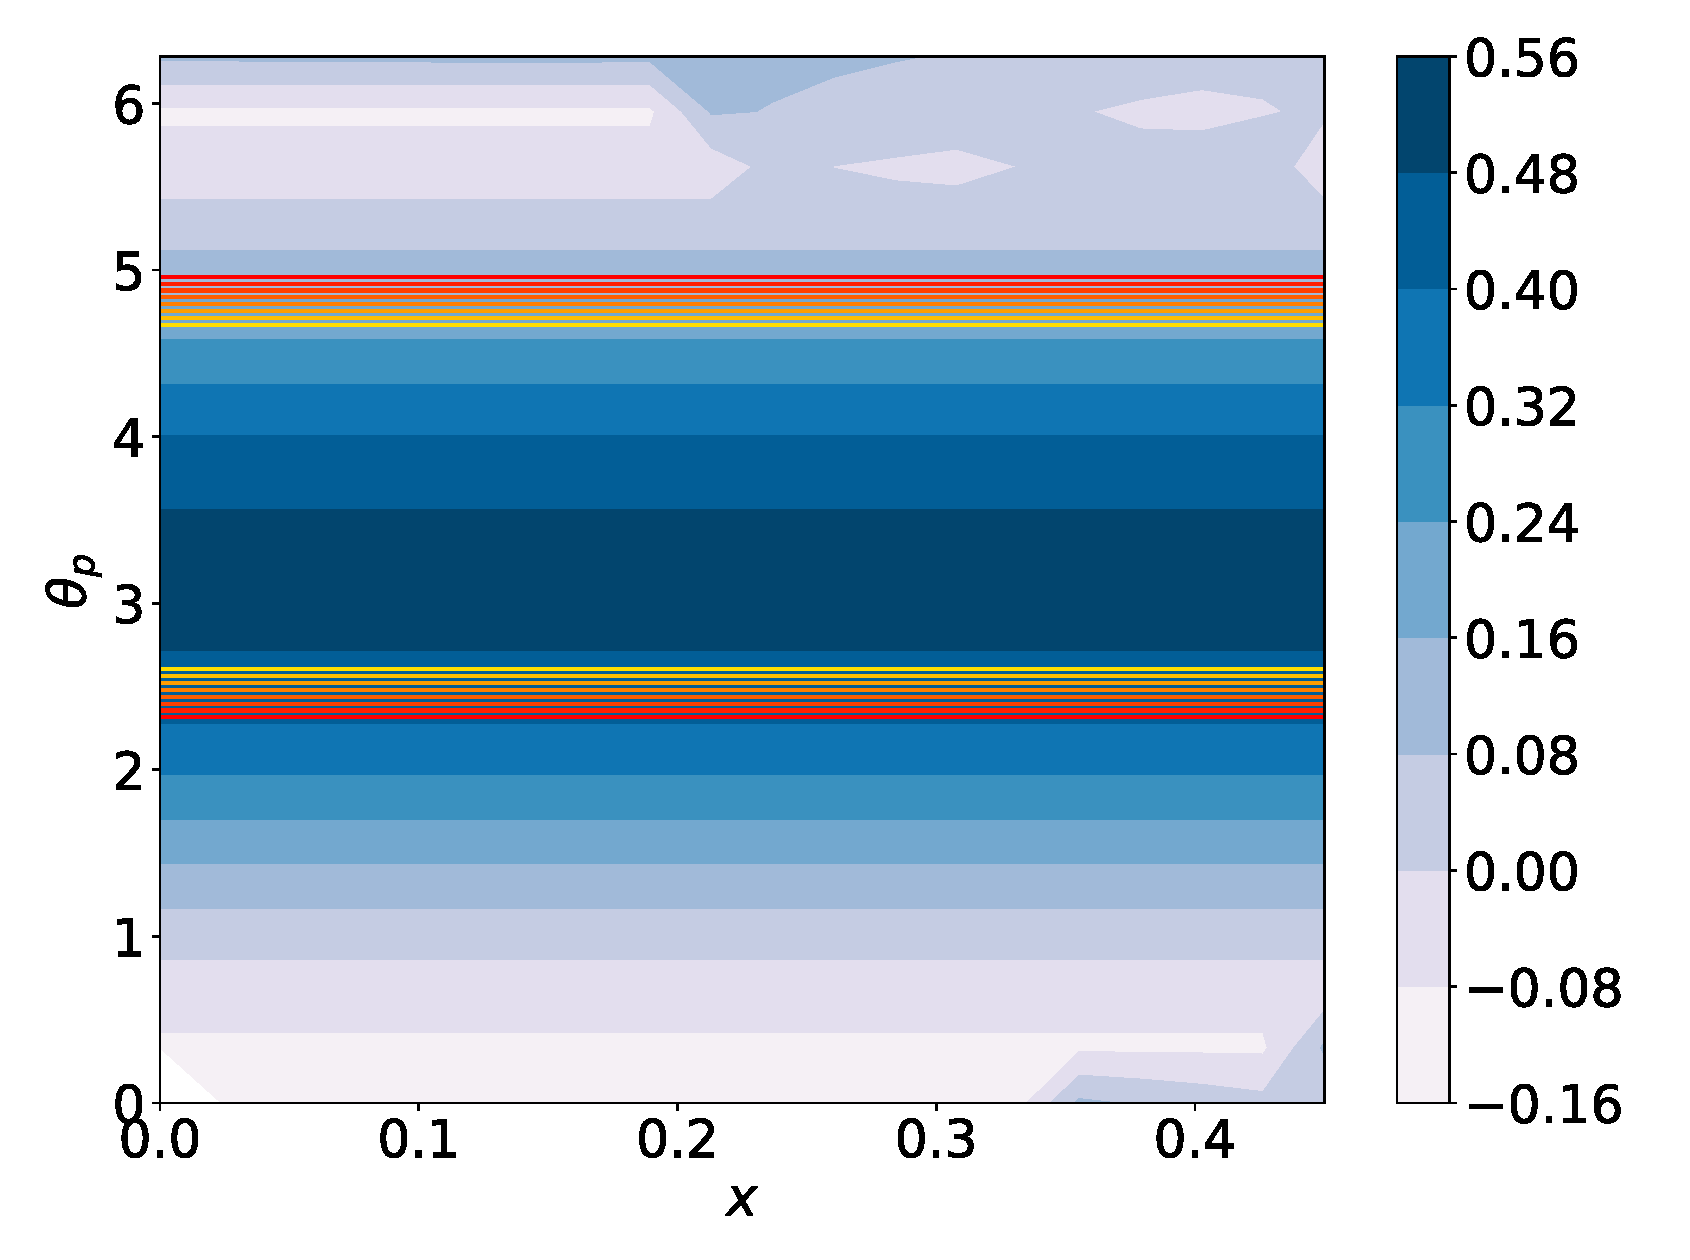
\includegraphics[width=1.0\linewidth]{gapContourAndBins.eps}
    \caption{Control switching as a function of gap function. There are total of two experts, one is active between the red boundaries}
    \label{fig:gapContour}
\end{figure}

\begin{figure}[H]
    \centering
    \includegraphics[width=1.0\linewidth]{cropped_MOE.png}
    \caption{Top row: Pendulum swing-up before impact. Bottom row: Velocity jump and control switching at impact}
    \label{fig:cartpole_trajectory}
\end{figure}


